\documentclass[11pt]{article}

\usepackage[margin=1in]{geometry}
\usepackage{amsfonts, amsmath, amssymb}
\usepackage{fancyhdr, float, graphicx}
\usepackage[utf8]{inputenc} % Required for inputting international characters
\usepackage[T1]{fontenc} % Output font encoding for international characters
\usepackage{fouriernc} % Use the New Century Schoolbook font
\usepackage[nottoc, notlot, notlof]{tocbibind}
\usepackage{listings}
\usepackage{xcolor}
\usepackage{blindtext}
\usepackage{hyperref}
\hypersetup{
	colorlinks=true,
	linkcolor=black,
	filecolor=magenta,
	urlcolor=blue,
	pdfpagemode=FullScreen,
}

\definecolor{codegreen}{rgb}{0,0.6,0}
\definecolor{codegray}{rgb}{0.5,0.5,0.5}
\definecolor{codepurple}{rgb}{0.58,0,0.82}
\definecolor{backcolour}{rgb}{0.95,0.95,0.92}

\lstdefinestyle{mystyle}{
	backgroundcolor=\color{backcolour},
	commentstyle=\color{codegreen},
	keywordstyle=\color{magenta},
	numberstyle=\tiny\color{codegray},
	stringstyle=\color{codepurple},
	basicstyle=\ttfamily\footnotesize,
	breakatwhitespace=false,
	breaklines=true,
	captionpos=b,
	keepspaces=true,
	numbers=left,
	numbersep=5pt,
	showspaces=false,
	showstringspaces=false,
	showtabs=false,
	tabsize=2
}

\lstset{style=mystyle}

% Header and Footer
\pagestyle{fancy}
\fancyhead{}
\fancyfoot{}
\fancyhead[L]{\textit{\Large{Blockchain Technology}}}
\fancyhead[R]{\textit{Krishnaraj T}}
\fancyfoot[C]{\thepage}
\renewcommand{\footrulewidth}{1pt}

\begin{document}

\begin{titlepage}
	\centering

	%---------------------------NAMES-------------------------------

	\huge\textsc{
		MIT World Peace University
	}\\

	\vspace{0.75\baselineskip} % space after Uni Name

	\LARGE{
		Attack Research and Documentation\\
		Fourth Year B. Tech, Semester 8
	}

	\vfill % space after Sub Name

	%--------------------------TITLE-------------------------------

	\rule{\textwidth}{1.6pt}\vspace*{-\baselineskip}\vspace*{2pt}
	\rule{\textwidth}{0.6pt}
	\vspace{0.75\baselineskip} % Whitespace above the title

	\huge{\textsc{
        My Ether Wallet and Ganache
    }} \\

	\vspace{0.5\baselineskip} % Whitespace below the title
	\rule{\textwidth}{0.6pt}\vspace*{-\baselineskip}\vspace*{2.8pt}
	\rule{\textwidth}{1.6pt}

	\vspace{1\baselineskip} % Whitespace after the title block

	%--------------------------SUBTITLE --------------------------	

	\LARGE\textsc{
		Lab Assignment 4
	} % Subtitle or further description
	\vfill

	%--------------------------AUTHOR-------------------------------

	Prepared By \vspace{0.5\baselineskip} % Whitespace before the editors

	\Large{
		Krishnaraj Thadesar \\
		Cyber Security and Forensics\\
        Batch A1, PA 15
	}

	\vspace{0.5\baselineskip} % Whitespace below the editor list
	\today

\end{titlepage}

\tableofcontents
\thispagestyle{empty}
\clearpage

\setcounter{page}{1}

\section{Aim}
The aim of this lab assignment is to understand the basics of Solidity programming and to develop simple smart contracts. This includes setting up the development environment, writing and deploying smart contracts, and interacting with them using MyEtherWallet and Ganache. The assignment will help in gaining practical experience in blockchain technology and smart contract development.

\section{Screenshots}

\begin{figure}[H]
    \centering
    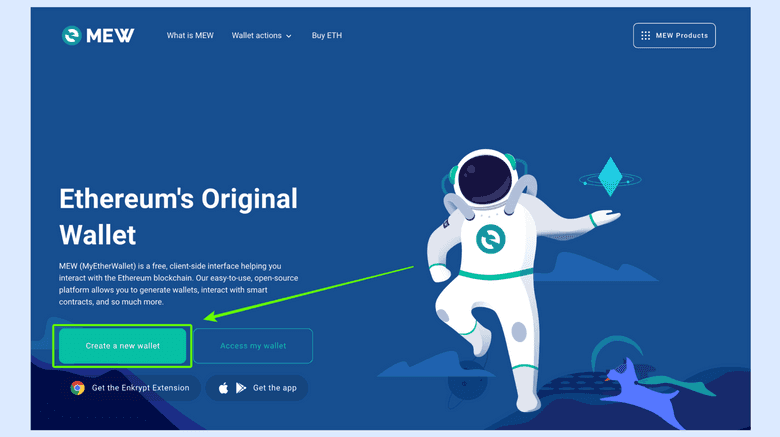
\includegraphics[width=0.8\textwidth]{1.png}
    \caption{My Ether Wallet}
    \label{fig:1}
\end{figure}

\section{Frequently Asked Questions}

\subsection{What is MyEtherWallet and how to set it up?}

MyEtherWallet (MEW) is an open-source, client-side tool for generating and managing Ethereum wallets. It allows users to create wallets, interact with smart contracts, and send transactions without relying on centralized exchanges.

To set up MyEtherWallet:
\begin{enumerate}
    \item Visit the official website: \url{https://www.myetherwallet.com/}.
    \item Click on “Create a New Wallet” and select a preferred method (e.g., Keystore file, mnemonic phrase, or hardware wallet).
    \item Follow the security guidelines to save your private key safely.
    \item Access the wallet using the chosen method and start managing Ethereum assets.
\end{enumerate}

\subsection{How to connect MyEtherWallet to the Ganache Network?}

To connect MyEtherWallet to Ganache:
\begin{enumerate}
    \item Open MyEtherWallet and go to the “Networks” section.
    \item Click on “Add Custom Network” and enter the following details:
    \begin{itemize}
        \item \textbf{Network Name:} Ganache Test Network
        \item \textbf{New RPC URL:} \texttt{http://127.0.0.1:7545} (default Ganache RPC URL)
        \item \textbf{Chain ID:} 1337 (or any custom ID from Ganache settings)
        \item \textbf{Currency Symbol:} ETH
        \item \textbf{Block Explorer URL:} (Leave blank for local Ganache)
    \end{itemize}
    \item Save the network settings and switch to the Ganache network.
\end{enumerate}

\subsection{How to import a Ganache account into MyEtherWallet?}

To import a Ganache account into MyEtherWallet:
\begin{enumerate}
    \item Open Ganache and copy the private key of an account.
    \item Open MyEtherWallet and select “Access My Wallet.”
    \item Choose “Software” and then “Private Key” as the access method.
    \item Paste the copied private key and unlock the wallet.
    \item You should now see the imported Ganache account with a test balance.
\end{enumerate}

\subsection{How to send a transaction on the Ganache network using MyEtherWallet?}

To send a transaction on the Ganache network using MyEtherWallet:
\begin{enumerate}
    \item Ensure that MyEtherWallet is connected to the Ganache network.
    \item Access the imported Ganache account.
    \item Click on “Send Transaction” and enter the recipient’s address (another Ganache account).
    \item Specify the amount of ETH to send.
    \item Adjust gas fees (optional, but typically unnecessary for Ganache).
    \item Click “Send” and confirm the transaction.
    \item Verify the transaction in Ganache’s transaction log.
\end{enumerate}

\subsection{How to get more Ether in Ganache for testing?}

Ganache provides pre-funded accounts with test Ether. If more is needed:
\begin{enumerate}
    \item Restart Ganache to reset the accounts and refill balances.
    \item If using Ganache CLI, start it with a higher initial balance:
    \begin{verbatim}
    ganache-cli --accounts 10 --defaultBalanceEther 10000
    \end{verbatim}
    \item Use \texttt{web3.js} or \texttt{truffle console} to transfer Ether between test accounts.
    \item Manually modify account balances in Ganache settings (if using GUI).
\end{enumerate}

\section{Conclusion}

MyEtherWallet provides a user-friendly interface for managing Ethereum accounts, interacting with smart contracts, and sending transactions. By integrating it with Ganache, developers can simulate real-world Ethereum transactions in a local test environment. This setup helps in smart contract testing and blockchain application development without incurring real-world gas fees.


% \begin{figure}[H]
%     \centering
%     \includegraphics[width=0.8\textwidth]{}
%     \caption{}
%     \label{fig:1}
% \end{figure}


\clearpage
\begin{thebibliography}{99}
\bibitem{ethereum}
Ethereum, \emph{Ethereum Whitepaper}, Available: \url{https://ethereum.org/en/whitepaper/}, Accessed: 2023-10-01.

\bibitem{ganache}
Truffle Suite, \emph{Ganache Documentation}, Available: \url{https://www.trufflesuite.com/ganache}, Accessed: 2023-10-01.

\bibitem{myetherwallet}
MyEtherWallet, \emph{MyEtherWallet Documentation}, Available: \url{https://www.myetherwallet.com/}, Accessed: 2023-10-01.

\bibitem{solidity}
Solidity, \emph{Solidity Documentation}, Available: \url{https://docs.soliditylang.org/}, Accessed: 2023-10-01.

\bibitem{web3js}
Web3.js, \emph{Web3.js Documentation}, Available: \url{https://web3js.readthedocs.io/}, Accessed: 2023-10-01.
\end{thebibliography}

\end{document}